   La situation peut être schématisée en dessinant un arc de cercle pour le 27\up{e} parallèle puisque les îles Rapa Nui et Rapa Iti sont toutes les deux situées sur ce parallèle.
   \begin{center}                        
      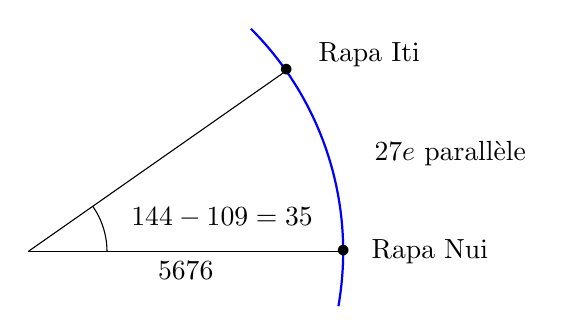
\begin{tikzpicture}
         \draw[blue, thick][samples=100,domain=-10:{144-109+10}] plot({4*cos(\x)},{4*sin(\x)}) ;
         \draw({5.5*cos(13)},{5.5*sin(13)}) node{\blue $27\up{e}$ parallèle};
         \draw (4,0) -- (0,0) node[midway, below]{$\ukm{5676}$};
         \draw (0,0) -- ({4*cos(35)},{4*sin(35)});
         \draw (5.1,0)node{Rapa Nui};
           \draw (4,0)node{$\bullet$};
         \draw  ({5*cos(30)},{5*sin(30)}) node{Rapa Iti};
         \draw  ({4*cos(35)},{4*sin(35)}) node{$\bullet$};
         \draw [samples=100,domain=0:{35}] plot({1*cos(\x)},{1*sin(\x)}) ;
         \draw ({2.5*cos(10)},{2.5*sin(10)}) node {$\udeg{144}-\udeg{109} =\udeg{35}$};
      \end{tikzpicture}                        
   \end{center}                
   La distance entre les deux îles représente une proportion de $\dfrac{35}{360}$ de la longueur du $27\up{e}$ parallèle qui est un cercle. \\
   Or, ce parallèle a une circonférence de $\ell =2\times\pi\times\ukm{5676} =11\,352\,\pi\,\ukm{}$. \\
   Par conséquent, la distance recherchée $d$ vaut : \\
   $d =\dfrac{35}{360}\times11\,352\,\pi\,\ukm{} \approx \ukm{3467,2711}$ \\                                        
   {\blue Les premiers navigateurs ont parcouru environ $\ukm{3467}$ entre ces deux îles}.
